\section{Target System}

The target system used for RG-D is the Hall B cryo target.~This target system has just been assembled and will be used first by RG-D experiments.~RG-D will use the following targets inside the Hall B cryo target system:

\begin{itemize}
\item	Liquid:
   \begin{itemize}
	\item	Hydrogen
	\item	Deuterium
    \end{itemize}
\item		Solid
   \begin{itemize}
	\item	Carbon
	\item	Copper
	\item	Tin
   \end{itemize}
\end{itemize}

The target configuration includes a 5 cm long liquid cell for Hydrogen or Deuterium (LD2), plus a solid target flag system, as shown in Fig.~\ref{fig:rgd-target} below. The flag system holds 2 carbon targets in series or a copper and a tin target in series.  The flag system is mounted in series with the liquid cell. The flag system can be remotely operated to put the carbon targets in the beam, no solid targets in the beam, or the copper and tin targets in the beam.

\begin{figure}\centering
  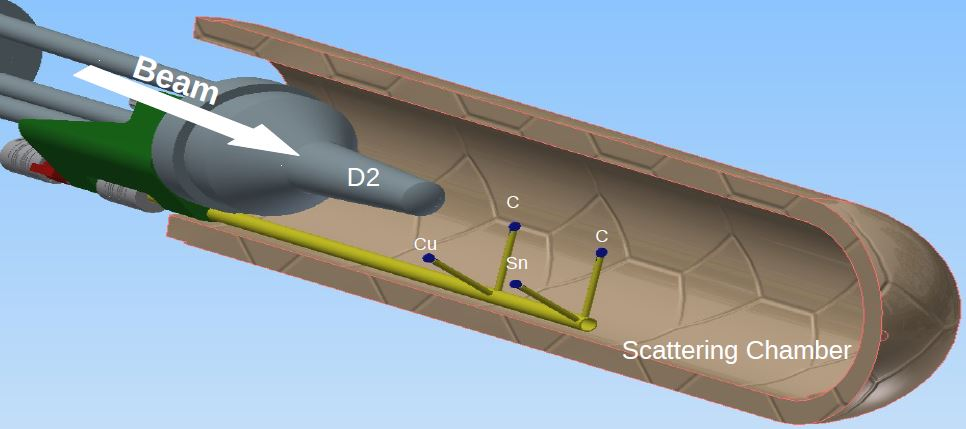
\includegraphics[width=\textwidth]{pics/rgd-target.jpg}
  \caption{The flag design with the 5 cm apart foils mounted on the same shaft (bottom yellow rod) with $\approx$ 55 degrees opening between their holding yellow needles that rotate together with a stepper motor. Each set of two foils will be inserted in the beamline in series with an empty LD2 target.\label{fig:rgd-target}}
\end{figure}

The targets are housed in a vacuum vessel along with the cryogenic system. A scattering chamber is installed around the target cell area. This is made from Rohacell foam with a wall thickness of 6.5 mm. Aluminum windows are used at the entrance and exit of the liquid cells, and at the exit of the scattering chamber. The details of all components, such as windows and cells, are shown on the beam line drawing, including thicknesses and locations. The beam line drawings can be found at \href{https://clasweb.jlab.org/wiki/index.php/User:Cwiggins}{https://clasweb.jlab.org/wiki/index.php/User:Cwiggins}.

\subsection{Hazards} 

The cryogenic target contains a condensed cryogenic fluid and is considered a pressure vessel. Sudden warming of the target due to a vacuum breach could result in rapid expansion of the target fluid. The system is designed to safely vent the excess pressure. Failure of the foam scattering chamber, or the thin window of the scattering chamber could produce a loud noise and could result in a failure of the target integrity.

The target utilizes flammable gas (hydrogen) during operation. Failure of the system could release flammable gas into the hall. The target gases and the helium used in the target refrigerator are potential ODH risks, and failure of either system could reduce the oxygen levels in the hall.

The target cell system is protected by 15 psi relief valves.  The target operates in a vacuum chamber, so the total pressure difference possible across the cell is 15~psi~+~14.7 ~psi=~29.7~psi. The cell is considered a pressure vessel. If the Kapton cell ruptures, the target gas would vent into the target vacuum space and the vacuum pumps would turn off. If the vacuum space pressure increases to 1 psi, the target gas will go out of the vacuum space relief valve and be discharged out of the Hall. No target gas would enter the Hall.

\subsection{Mitigations}

The design and construction of the entire Hall B cryo target is in accordance with AMSE standards. During operation, the foam scattering chamber, and the thin window are surrounded by the Hall-B CLAS12 Central Detectors and are therefore difficult to access.~A protective shield will be placed around the scattering chamber whenever the target is retracted from the Central Detector system and is under vacuum.  Personnel working near the target shall wear hearing and eye protection whenever the foam extension and window are exposed and the system is under vacuum. No cold cryogenic components are accessible by personnel.

Relief valves are installed in all the target pressure circuits so the safety system is entirely passive.~The quantity of flammable gas (H2) is less than 80~g and is therefore considered a class-O installation (!600~g) and the rules and regulations for this installation shall be followed, notably:

\begin{itemize}
\item The area shall be posted ``Danger Flammable Gases. No Ignition Sources" 
\item Combustibles and ignition sources shall be minimized within 10 ft or 3~m of target’s gas handling equipment and piping.
\end{itemize}

The target does not operate in a confined space, and the total quantity of hydrogen/helium in the system is under 1000 standard liters. This presents a negligible oxygen deficiency risk in Hall B and therefore is a class-0 ODH installation.  Hydrogen shall be loaded into the system by qualified personnel only, and those personnel shall follow approved operational gas handling procedures.

The target control software includes numerous alarms (temperature, pressure, vacuum, heater power, etc.) to alert users to potential problems.

\subsection{Responsible Personnel}

The target system will be maintained by the JLab Target Group.  

\begin{table}[!htb]
\centering
\begin{tabular}{|c|c|c|c|c|}
\hline
 Name&Department.&Phone&email&Comments \\ \hline
Xiangdong Wei & Hall B &(757) 871-5374&\href{mailto:xwei@jlab.org}{\nolinkurl{xwei@jlab.org}} &1st contact \\ \hline
Engineering on call & Hall~B&(757)-748-5048&& 2nd contact  \\ \hline
\end{tabular}
\caption{Personnel responsible for the CLAS12 target system.} 
\label{tb:target}
\end{table}
